\chapter{Introduction}
  \section{Overview}
  Microseconds after the Big Bang, the Universe existed in a state known as
    the Quark Gluon Plasma (QGP).
  In the QGP, quarks and gluons are not in hadronic bondage, forced to 
    the confines of bound states such as protons and neutrons.
  The Large Hadron Collider (LHC) produces QGP in the lab in lead-lead (PbPb)
    collisions.
  The high energies and rates of the collisions at the LHC make it possible 
    to do detailed studies of the QGP. 
  The LHC is producing rare experimental probes such as suppressed jets and 
    heavy quarkonia at unprecedented rates in heavy-ion collisions. 
  As a result of recent LHC studies described in this thesis, physicists now 
    have better constraints on the QGP properties like temperature, viscosity, 
    and energy density.

  The detailed studies of PbPb collisions coming out of the LHC 
    experiments are in need of a understanding of the initial state of the ions 
    before they collide.
  Without more knowledge of the initial state, physicists cannot determine 
    which experimental effects are due to the QGP and which effects are 
    inherent to the nuclei themselves. 
  For example, suppression of heavy quarkonia is a signature of the QGP 
    but also appears to occur in deuterium-gold (dAu) collisions where the QGP 
    is not expected to arise \cite{dAuOniaPHENIX}. 
  Another important example is the measurement of viscosity, which depends on 
    the relationship between the observed azimuthal anisotropy and the 
    initial eccentricity of the overlap of the two colliding nuclei 
    (see Section~\ref{sec:elipFlow}). 
  A clean probe of the initial state is needed by physicists to comprehensively 
    understand the QGP.
  Ultra-peripheral heavy-ion collisions (UPC) at the LHC provide such a probe.

  The current understanding of heavy-ion collisions evolved over the
    last 30 years.
  Relativistic heavy-ion collisions were first studied using the 
    Alternating Gradient Synchrotron (AGS) at Brookhaven National Lab (BNL) 
    in Upton, NY, followed by the Super Proton Synchrotron (SPS) at CERN near 
    Geneva, Switzerland. 
  From the numerous AGS and SPS experiments two main observables emerged,
    namely, \JPsi{} suppression and strangeness enhancement \cite{sps}. 
  These results pioneered the search for the QGP. 

  At AGS the ion isotopes $^{16}$O, $^{28}$Si, and $^{197}$Au beams were 
    collided with fix targets. 
  At SPS the same fix target configuration was used, but the ion isotopes were 
    $^{16}$O, $^{32}$S, and $^{208}$Pb.
  The center of mass energies per nucleon pair, $sqrt{s_{NN}}$, for these 
    experiments ranged from just below 5 GeV to 20 GeV. 
  Although the strangeness enhancement and \JPsi{} suppression 
    signals indicated that a deconfined state of quarks and gluons was likely 
    created, at the energies of the AGS and SPS this state perished quickly. 
  The threshold for creating the QGP requires an energy density of $\sim$ 0.15 
    GeV/$fm$$^{3}$ and a temperature near 170 MeV \cite{qgpThresh}.
  Because of this, the QGP signals at the AGS and SPS energies could 
    not have lasted long enough to study their properties. 

  Plans for a colliding beam machine dedicated to heavy-ions, designed to reach 
    energies of 200 GeV per nucleon pair, was first proposed in 1983.
  It was believed that in these collisions signs of a hot gas of quarks and 
    gluons would emerge.
  In 2000, RHIC began collisions and the four experiments,
    STAR, PHENIX, BRAHMS, and PHOBOS started taking data. 
  The energies at RHIC were a factor of 10 higher than was previously achieved
    reaching the designed maximum energy. 
  RHIC experiments confirmed the existence of a  thermalized state of quarks and 
    gluons.
  Contrary to expectations, the state found at RHIC was found to be 
    a strongly coupled fluid with nearly no viscosity \cite{whi}.

  The LHC heavy-ion program began collisions in 2010, colliding PbPb at 
    a center of mass energy of 2.76 TeV per nucleon pair. 
  This corresponds to an increase in the colliding energy by an order of 
    magnitude with respect to RHIC. 
  The LHC experiments, ALICE, ATLAS, and CMS have been studying the heavy-ion 
    collisions since then. 
  In 2013 LHCb joined the LHC heavy-ion program. 
  Thanks to the LHC and RHIC physics programs, a new era of precision
    heavy-ion measurements is underway. 
  The latest results from the LHC have come from the 2013 proton-lead (pPb)
    run.
  This period of data taking was originally designed to be a control 
    measurement.
  However, CMS and ALICE have both shown an elliptical flow-like signal present
    in the pPb data \cite{}, which was unexpected.
  Understanding the origin of this nuclear effect is one of the most important
    priorities of the heavy-ion physics program at present. 
  The latest data from the pPb measurements confirm the need to 
    understand the nature of the initial state. 
  UPC events fulfill this need by probing the nucleus through photon 
    interactions.
  By measuring UPC \JPsi{} events, theoretical models of the initial state can 
    be constrained.
  In this thesis, the CMS capability for measuring this process, the 
    description of the analysis, and the comparison between the measured 
    coherent \JPsi{} cross section to theoretical models are given. 

  In this chapter, the measurement of transverse energy, direct photons, and
    elliptic flow will be discussed.
  The transverse energy and direct photons measurements are related to 
    the energy density and temperature of the QGP, which provide a 
    confirmation of the production of QGP.
  The elliptic flow measurement is related to the viscosity of the QGP, which
    provides insight into the fluid like nature of the QGP state.
  Before discussing these results, several terms used to describe heavy-ion
    measurements and detectors will be discussed. 
  This discussion will be divided into two parts, a generic description of 
    the main detector elements, and an explanation of variables used in
    heavy-ion measurements.
  
  \section{Variables in heavy-ion measurements}
    The variables used by heavy-ion experiments at colliding beam facilities, 
      such as the LHC and RHIC, are due to the cylindrical configuration of 
      the detectors around the line of the beams.
    Two types of generic detectors are in use in heavy-ion experiments, 
      trackers and calorimeters. 
    A tracker measures the trajectory of the particles as they pass through 
      the detector.
    The particle trajectories measured by a tracker detector are called 
      tracks.
    From these tracks, the particles' momenta can be deduced. 
    In CMS tracks are mapped out from measuring charge deposits of in silicon
      cells.
    A tracker will typically be designed to interact minimally with the 
      particles in order to preserve the trajectories of the particles. 
    The second generic type of detector, a calorimeter, records the energy 
      of the particles that hit it. 
    A calorimeter is typically filled with dense material used to initiate a 
      shower of particle collisions.
    The light from this shower of particles is collected and used to measure 
      the energy of the initial particle or particles which hit the 
      calorimeter.
    Unlike a tracker, a colorimeter typically is designed to stop the particles
      which hit it and collect as much of the energy of these particles as 
      possible.
    The details the CMS detector will be discussed in more detail in 
     Chapter~\ref{ch:detector}.

    Heavy-ion measurements will typically be comprised of 
      combinations of the variables, $p$, for momentum, $E$, for energy, 
      $\phi$, for the azimuthal angle, \pt, the transverse momentum, $y$, 
      for rapidity, and $\eta$, for pseudorapidity. 
    Energy are typically measured by a calorimeter and momentum by a tracker.
    The $\phi$ angle is measured around the beam axis. 
    The transverse momentum, \pt, is the component of the momentum that points
      perpendicular to the beam line. 
    Rapidity is related to energy and momentum by 
    $y$ = $\frac{1}{2}ln\left(\frac{E+p_{z}}{E-p_{z}}\right)$, where $p_{z}$ 
      is the momentum component that points in the direction of the beam axis. 
    Here $c$ is taken to be equal to 1. 
    Pseudorapidity is defined by
      $\eta=\frac{1}{2}ln\left(\frac{|\mathbf{p}|+p_{Z}}{\mathbf{p}|-p_{Z}}\right)$, 
      which can be shown to be equal to $-ln\left(tan\left(\theta/2\right)\right)$.
    If $m << p$, where $m$ is the mass of the particle, the 
      relativistic equation for energy, $E^2=p^2+m^2 \rightarrow E=p$, and 
      pseudorapidity is equal to the rapidity. 
    Tracker measurements will typically provide a rapidity value with 
      the mass assigned based on a particle identification criteria, where as 
      calorimeter based measurements will typically be assigned a rapidity 
      based the angle $\theta$ with respect to the interaction point.

    In addition, the variable called centrality is used in heavy-ion 
      collisions to characterize the degree of activity. 
    It is typically either measured using activity in either a calorimeter in
      the forward region at high $\eta$ values or by the number of tracks.
    Centrality is reported as a percentage where 0\% corresponds to the most 
      energetic collisions and 100\% corresponds to the least energetic.
    For example, events assigned a centrality between 0-10\% would be the 
      top ten percent of events in terms of number of hits in a tracker 
      detector or energy in a forward calorimeter depending on which 
      variable is used for centrality. 
    The number of nucleons that participate in a collision, $N_{part}$,
      the number of collisions between these participants, $N_{col}$, and the
      closest distance between the center of the two colliding nuclei, the 
      impact parameter, $b$, are all related to the measured centrality 
      percentage by use of a simulation. 
    The convention of labeling the most active centralities 0\% and the least
      active 100\% is due to the correlation between the impact parameter.
    When the nuclei collide exactly head on the impact parameter is 0, which 
      correlates with a 0\% centrality value. 

  \section{Temperature and energy density of the QGP}
    Lattice QCD predicts that the QPG forms above a critical temperature and 
      energy densities, 170 MeV and 1.5 GeV/$fm$$^{-3}$ \cite{}.
    The measurement of the $\frac{dE_{T}}{d\eta}$ provides a means of 
      estimating the energy density of the hot state created in heavy-ion
      collisions. 
    The value of $E_{T}$ for this measurement is defined as 
      $E_{T}=\sum_{i}E_{i}sin\theta_{i}$, where $E_{i}$ is the energy measured 
      by the ith calorimeter element and $\theta$ is the angle between the 
      center of the detector element and the interaction point. 
    The temperature can be estimated from the transverse momentum 
      spectrum of the direct photons, with are photons that are produced 
      directly from the QGP.
    The measurements from CMS and ALICE at the LHC and STAR and PHENIX at RHIC
      confirm that the critical values for energy density and temperature are
      exceeded.

    The values of $\frac{dE_{T}}{d\eta}$ measured by CMS \cite{cmsEt} and PHENIX 
      \cite{phenixDeDeta} were done using the experiments' calorimeter 
      systems.
    For the calculated $\frac{dE_{T}}{d\eta}$ at $\eta = 0$, the interval 
      $|\eta| > 0.35$ was used by both experiments and corresponds to the full
      coverage of the PHENIX calorimeters. 
    From the $\frac{dE_{T}}{d\eta}$ at $\eta = 0$ measurements, the energy 
      density of the created medium at the LHC and RHIC were estimated from the
      Bjorken energy density formula, 
    $\epsilon_{Bj}=\frac{1}{A\tau}\frac{dE_{T}}{dy}$, where $A$ is the region
      of overlap between the two colliding nuclei and $\tau$ is the formation
      time of the medium \cite{bjEdense}.
    The formation time times the energy density, $\tau\dot\epsilon_{Bj}$, 
      from PHENIX was measured at RHIC to be 5.4$\pm$0.6 GeV $fm$$^{-2}$c$^{-1}$ 
      for the centrality interval 0-5\% 
    At the LHC CMS measured $\tau\dot\epsilon_{Bj}$ = 14 GeV $fm$$^{-2}$c$^{-1}$ 
      for the same centrality interval.
    Both values are well above the critical energy density of about 1.5 GeV/$fm$$^{3}$ 
      calculated from lattice QCD when assuming a medium formation time $\tau$ 
      = 1 $fm$/$c$.
      \begin{figure}[!Hhbt]
        \centering
        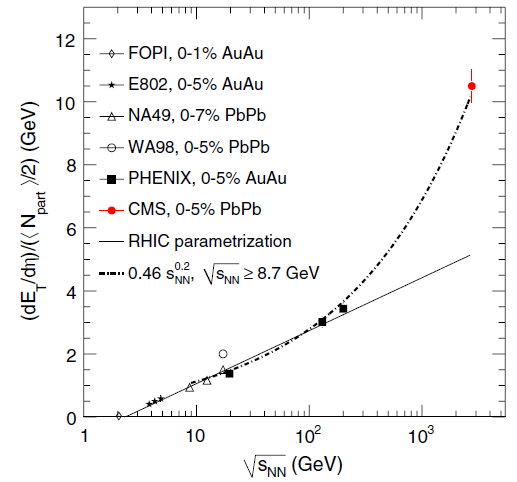
\includegraphics[width=.65\textwidth]{dEtdEta}
        \caption{Comparison of $\frac{dE_{T}}{d\eta}$ as a function of 
          collision energy, $\sqrt{s_{NN}}$, normalized by the number 
          participating nucleons, $N_{p}$, to account for the difference in 
          the ion species collided at the various different experiments.}
        \label{fig:dEtdEta}
      \end{figure}

    Direct photons defined as thermal photons created in the QGP, have been 
      measured at RHIC by PHENIX \cite{phenixPhoton2010} and at the LHC by ALICE 
      \cite{photonALICE} through the measurements of electron-positron pairs.
    Each experiment measured the inclusive \pt{} spectrum from 
      electron-positron pairs, all pairs from the sample are taken without
      regard to the creation mechanism.
    The PHENIX measurement was taken from pp collisions and top 20\% most 
      energetic AuAu collisions, collisions with a centrality of 0-20\%. 
    The ALICE measurement analyzed the 0-40\% centrality and 40\%-80\% centrality
      PbPb collisions, and pp collisions. 
    In the PHENIX and ALICE measurements, the contribution to the inclusive 
      spectrum was sorted into a direct component and a background component.
    The latter consists mainly of decays from hadrons such as $\pi$ and $\eta$
      particles. 
    In the PHENIX measurement this was done by fitting to the mass 
      distribution of the electron-positron pair for each \pt{}.
    For the ALICE measurement, the double ratio between the inclusive photons 
      to pions over the ratio between photons from hadron decays and pions was
      measured to estimate the direct contribution. 
    The inclusive photon \pt{} spectra were then rescaled by the direct 
      photon fractions.
    The slope of an exponential fit to the low \pt{} portion of the direct 
      photon spectrum is used to measure the temperature.
    \begin{figure}[!Hhbt]
      \centering
      $ \begin{array}{c c}
        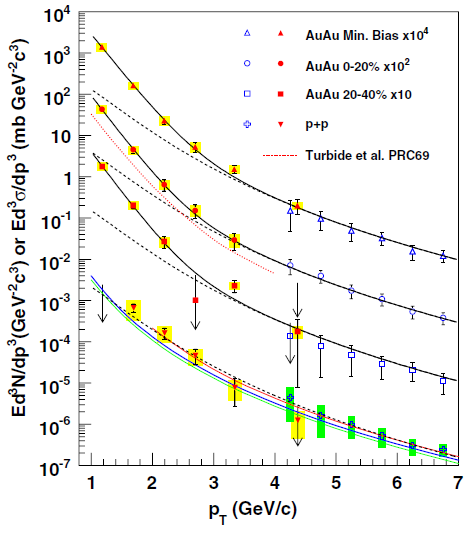
\includegraphics[width=.4\textwidth]{phenixDirectPhoton} &
        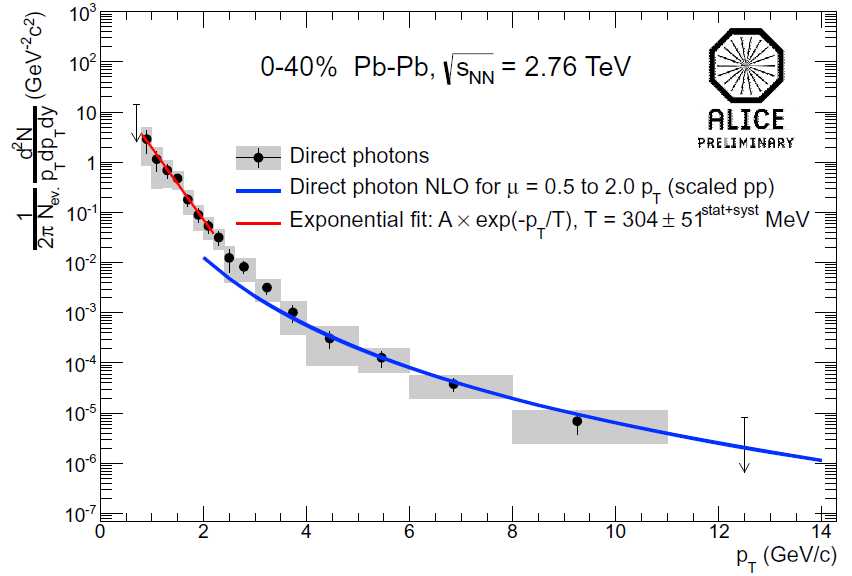
\includegraphics[width=.55\textwidth]{aliceDirectPhoton}
      \end{array} $
      \caption{Direct photon yield as a function of \pt{} from 
        PHENIX \cite{phenixPhoton2010} (left) and ALICE \cite{photonALICE} 
        (right)}
      \label{fig:directPhotonPt}
    \end{figure}

    The temperature obtained from direct photon measurements offers a clear
      way of establishing whether the critical temperature for deconfinement
      was achieved. 
    The direct photon \pt{} spectra in Fig.~\ref{fig:directPhotonPt} shows a 
      clear enhancement at low \pt{} compared to the rescaling to the pp 
      spectra that fits the high \pt{} part, indicating a clear deviation from 
      pp collisions.
    The low \pt{} photons are then consistent with thermal activity of
      the QGP.
    The thermal spectrum of the QGP is therefore imprinted on this part of 
      the spectrum.
    The temperature from PHENIX was measured to be 221 $\pm$ 21 MeV and 
      304 $\pm$ 51 MeV from ALICE, both well above the critical temperature
      estimated from lattice QCD of $\sim$ 170 MeV.
    The combination of the energy density and temperature measurements
      create a consistent picture, that both RHIC and the LHC have created a 
      deconfined state.

  \section{Elliptic flow and viscosity in the QGP \label{sec:elipFlow}}
    Prior to RHIC, the QGP was thought to be a hot gas of quarks and gluons.
    At RHIC, elliptic flow, $v_{2}$, was measured showing that the medium 
      appears to obey hydrodynamic equations and flows like a fluid.
    This same signal was also measured by CMS \cite{cmsFlow} at the LHC. 

    Elliptic flow is the second order Fourier expansion coefficient  
      of the azimuthal distribution of measured tracks.
    This expansion has the form
    \begin{equation}
      1+\sum^{\infty}_{n=1}2v_{n}\mathrm{cos}\left[n\left(\phi-\Psi\right)\right],
      \label{eg:v2Expand}
    \end{equation}
      where $v_{n}$ is the $n$th coefficient of the Fourier expansion, $\phi$
      is the azimuthal angle, and $\Psi$ is the event-plane angle.
    The event-plane angle accounts for the random orientation of the 
      nuclei event-by-event and is correlated with the reaction-plane
      , $\Psi_{R}$ (see Fig.~\ref{fig:elipSchem}).
    The reaction-plane is defined by the line which runs through the center
      of the two nuclei when they reach the distance of closest approach. 
    \begin{figure}[!Hhbt]
      \centering
      $ \begin{array}{cc}
      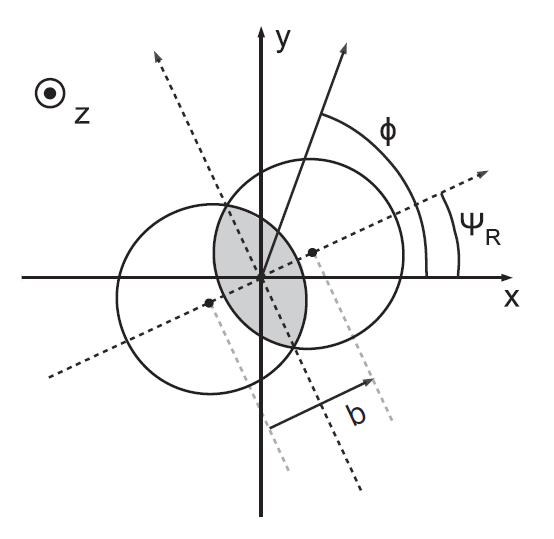
\includegraphics[width=.45\textwidth]{elipFlowSchemCMSGrey} &
      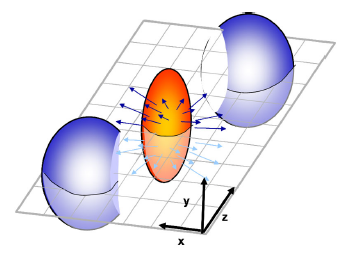
\includegraphics[width=.45\textwidth]{elipFlowSchem}
      \end{array} $
      \caption{Schematic of the initial nuclear overlap and elliptic flow.}
      \label{fig:elipSchem}
    \end{figure}

    The $v_{2}$ signal is believed to arise from pressure gradients.
    These pressure gradients originate from the initial elliptical shape of 
      the overlap region between the colliding nuclei. 
    The pressure gradient is higher along the shorter axis compared to 
      the longer axis of the ellipsoid in Fig~\ref{fig:elipSchem}.
    This difference in pressure gradient will create a flow of the QGP 
      medium in the direction of the shorter axis. 
    The flow is responsible for the measured anisotropic distribution of 
      tracks. 

    The extent to which the initial shape of the overlap translates to flow
      in the medium is controlled by viscosity. 
    A viscous fluid will tend to smooth out anisotropies and results in 
      a smaller flow signal for the same overlap configuration of the initial
      nuclei. 
    The ratio between the measured $v_{2}$ signal and the initial 
      eccentricity, $\epsilon$, based on the given centrality is sensitive
      to the viscosity of the medium. 

    \begin{figure}[!Hhbt]
      \centering
      $ \begin{array}{cc}
        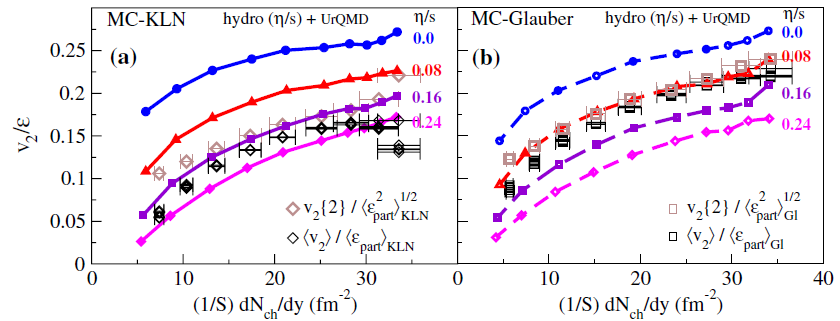
\includegraphics[width=.75\textwidth]{etaOvSinit} \\
        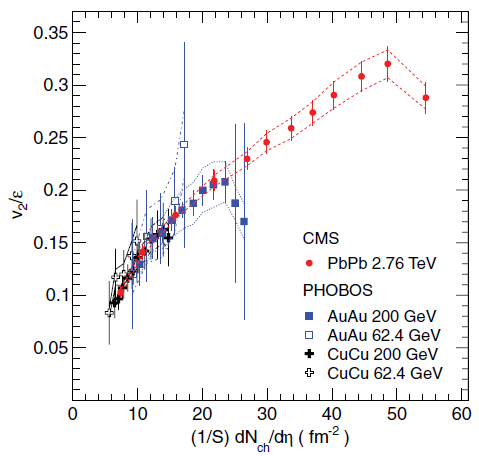
\includegraphics[width=.75\textwidth]{elipFlowCMS}
      \end{array} $
      \caption{$v_{2}/\epsilon$  as a function of $1/S \frac{dN_{ch}}{dy}$
        for different different values of $\eta/s$ for KLN initial state 
        (left) and Glauber initial state (center) compared to STAR (overlaid)
        and CMS and PHOBOS data (right).}
      \label{fig:elipFlow}
    \end{figure}

    In Fig.~\ref{fig:elipFlow}, $v_{2}/\epsilon$ is plotted as a function of 
      the number of charged particle, $N_{ch}$, per unit of pseudorapidity, 
      $\eta$, per area of overlap between the colliding nuclei, 
      $S$ \cite{etaOvSinit}. 
    The model calculation was performed for four values of the ratio of the 
      shear viscosity over entropy density, $\eta/s$, which are 
      0.0, 0.08, 0.16, and 0.24.
    The $\eta/s$ value which gives the best agreement with data in 
      Fig~\ref{fig:elipFlow} depends strongly on the initial state model 
      calculation.
    The observed strong dependence is one of the primary reason
      why more studies on the nature of the initial state are needed. 
    
  \section{Recent results from HI control measurements}
    The proton-nucleus runs at the LHC and RHIC were pursued as
      control measurements. 
    It was believed that these configurations could measure 
      initial state backgrounds to heavy-ion measurements.
    However, a flow-like signal has been very recently measured in pPb 
      collisions by LHC experiments.
    A $v_{2}$ signal, like that indicating flow of the QGP in PbPb collisions,
      has been measured by CMS \cite{}.
    \begin{figure}[!Hhbt]
      \centering
      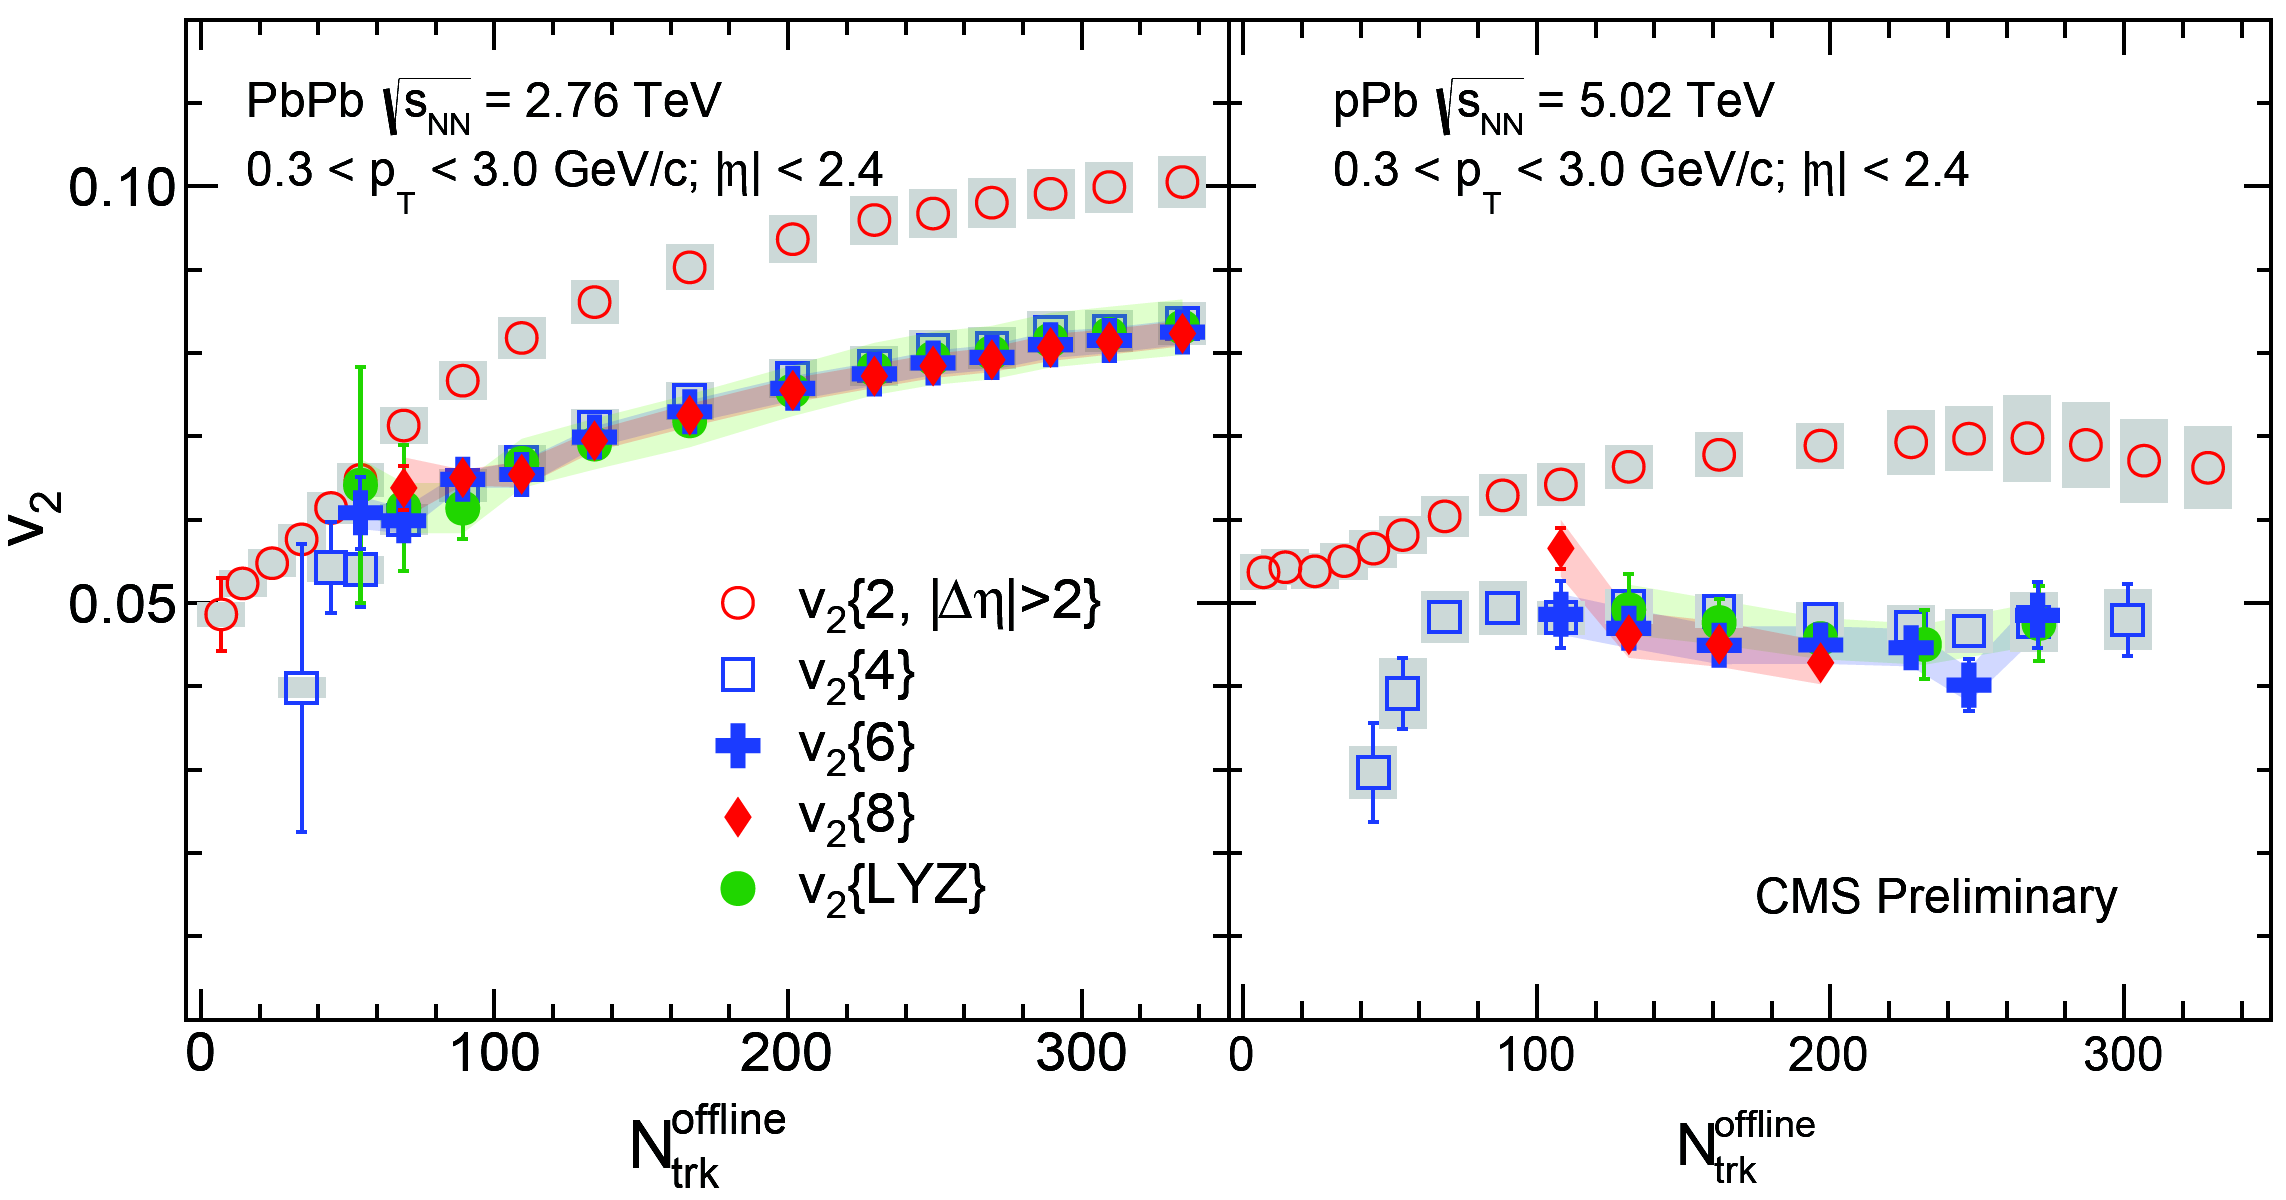
\includegraphics[width=.65\textwidth]{elipFlowCMSPPb}
      \caption{$v_{2}$ measured using the cumulant method in pPb collisions}
      \label{fig:pPbFlow}
    \end{figure}

    The $v_{2}$ measurement shown in Fig~\ref{fig:pPbFlow} uses a cumulant 
      method.
    This method differs from the event plan method discussed above, in that 
      it uses the correlations between tracks rather than the $\phi$ angle 
      of the tracks with respect to the events plan angle.
    This method can be done using the correlations between any number of 
      tracks. 
    The number of tracks that are used for a given method is 
      indicated by the number in brackets. 
    In addition a method called the Lee-Yang Zeros (LYZ) method was used, 
      which uses the correlations between all the tracks. 
    The measurement is done over a range of total number of track, 
      $N^{offline}_{trk}$. 
    The range shown in Fig.~\ref{fig:pPbFlow} corresponds to the number of 
      tracks present in PbPb collisions for centrality values between 50-60\%.
    The $v_{2}$ measurements using more than 2 track correlations are all 
      consistent with each other.
    This is an indication that $v_{2}$ in pPb collisions at the LHC is the
      result of collective motion.
    The pPb $v_{2}$ measurement underscores the need for a clean probes of the initial 

    In this thesis the analysis of ultra-peripheral \JPsi{} photoproduction 
      is discussed. 
    In UPC events, the interaction between the nuclei occurs through
      exchange of photons. 
    This results in a clean probe of the initial state of the nucleus.
    In the following chapter, the theory of \JPsi{ } photoproduction in 
      UPC events is presented. 
    
